\documentclass[11pt, fleqn]{article}

\usepackage[usenames,dvipsnames,svgnames,table]{xcolor}
\usepackage{amsmath}
\usepackage{amsfonts}
\usepackage[margin=1in]{geometry} % To set the margin widths
\usepackage{graphicx}
\usepackage{listings}
\usepackage{multirow}
\usepackage{tabularx}
\usepackage{varioref}
\usepackage[noabbrev,capitalize]{cleveref}
\usepackage[group-separator={,}]{siunitx}
\usepackage{subcaption}
\usepackage{titlesec}
\usepackage{lscape}
\usepackage{bm}
\usepackage{chngpage}
\usepackage[titletoc,toc,title]{appendix}

\renewcommand\thesection{\arabic{section}}
\renewcommand\thesubsection{\thesection\alph{subsection}}

\lstset{
  frame=single,
  basicstyle=\ttfamily,% print whole listing small
  language=R,
  aboveskip=3mm,
  belowskip=3mm,
  showstringspaces=false,
  columns=flexible,
  numbers=none,
  commentstyle=\color{ForestGreen},
  stringstyle=\color{Maroon},
  breaklines=true,
  breakatwhitespace=true,
  tabsize=2,
  literate={<-}{{$\gets$}}1 {~}{{$\sim$}}1
}

\sisetup{output-exponent-marker=\textsc{e}}

\setlength{\parskip}{12pt} % Sets a blank line in between paragraphs
\setlength\parindent{0pt} % Sets the indent for each paragraph to zero

\begin{document}

\title{Homework \#3\\
Digital and Algorithmic Marketing (37304-01)}
\author{
Brian Chingono, Will Clark, Matthew DeLio, Jonathan Stevens (\textbf{Group \#8})\\
University of Chicago Booth School of Business}

\maketitle

\section{Gender-Based Preferences of Message Senders}

\vref{fig:heatmap_female,fig:heatmap_male} show, for a given sender rating, the difference between the conditional probability of sending a message (conditioned on the senders rating) and the marginal probability of sending a message across all receiver ratings. 

To take a concrete example from \cref{fig:heatmap_female}: suppose I am a female with a rating of 6. I am 2.2 percentage points more likely to target a man with a rating of 7 than the average woman is. Formally:
\[ Pr(\text{message}|F=7,M=6) - Pr(\text{message}|M=6) = 2.2 \text{ percentage points}\]

\doublefig{}{heatmap_female}{Relative Preferences of Female Senders}{heatmap_male}{Relative Preferences of Male Senders}

A few random observation:
\begin{itemize}
\item It pays to be an average-looking woman, but not an average-looking man. Conditional on their own ratings, men are slightly more likely to reach out to a woman who is rated  6, while women are slightly less likely to reach out to men who are rated 6. 
\item The pattern reverses for those receivers who are rated slightly above average. Men are less likely to reach out to a woman who is rated a 7, while women are more likely to reach out to a man who is rated a 7.
\item In general, men and women both tend to aim for partners who are rated similar to themselves. This is why we see positive numbers concentrated on the diagonal axis in \cref{fig:heatmap_female} and \cref{fig:heatmap_male}. As a rule, though, men are likely to aim a little higher (or lower!) than women. 
\end{itemize}

We can formalize this last point with a regression:
\[ R_{i,j} = \alpha_j + \beta_j S_{i,j} + \varepsilon_{i,j} \]
where $R_{i,j}$ is the rating of receiver $i$, $S_{i,j}$ is the rating of sender $i$, and $j=\text{\{female,male\}}$. Essentially we are trying to predict the rating of the receiver given the rating of the sender.

The estimated intercept will tell us what is the unconditional expectation for the receivers' ratings. The estimated slope coefficient will tell us the degree to which men or women target those with similar ratings. The higher the coefficient, the more likely it is that senders target similarly rated receivers (i.e. if $\hat{\beta}=1$ then people would only message those who are rated exactly the same as themselves).

% latex table generated in R 3.2.3 by xtable 1.8-2 package
% Mon Apr 25 21:30:19 2016
\begin{table}[ht]
\centering
\caption{Regressing Receiver Looks on Sender Looks} 
\label{tab:receiver_on_sender}
\begin{tabular}{rrrr}
  \hline
 & $\alpha_j$ & $\beta_j$ & R-squared \\ 
  \hline
Female senders & 5.17 & 0.209 & 0.0466 \\ 
  Male senders & 5.94 & 0.159 & 0.0263 \\ 
   \hline
\end{tabular}
\end{table}


For both genders, the unconditional expectation of the receivers' rating is below average (given that the average is a 6). Somewhat surprisingly, women (on average) tend to send messages to men who are slightly \textit{better} looking than they are, while men (on average) send messages to women who are slightly \textit{worse} looking than they are.\footnote{The rating of the average female sender is 5.05 (lower than $\hat{\alpha}_{F}$); the rating of the average male sender is 5.32 (higher than $\hat{\alpha}_{M}$).} Given that the coefficient $\hat{\beta}$ is higher for women than for men, in the aggregate, women are more likely than men to target someone who is rated similarly. Note, however, that the R-squared values for both regressions are very low, so this simple model explains very little of the targeting preferences for either gender.

We can see this most clearly in \vref{fig:dotplot_female,fig:dotplot_male}. The volume of messages for a given receiver/sender pair are plotted (bigger dots $\rightarrow$ more messages). Women tend to be a little more discriminating than men, as the bulk of the messages seem to be slightly more concentrated near the diagonal axis. The regression line for each gender is plotted, and we can see that the line for women is a little bit steeper (though not by much!) than the line for the men.


\doublefig{}{dotplot_female}{Aggregate Sending Behavior of Females}{dotplot_male}{Aggregate Sending Behavior of Males}


\section{}


\section{}
We created an 11 x 11 matrix with the match scores that are associated with different combinations of male looks and female looks. \vref{fig:q3_score_heatmap} shows a heatmap of the results. The red cells indicate low match scores and the blue cells represent high match scores. 

Across the entire matrix, the average match score is 0.088. Overall, the following observations can be made from \cref{fig:q3_score_heatmap}:
\begin{itemize}
\item The most attractive women (categories "11" and "10") have above-average match scores, regardless of the appearance of their male counterpart. For example, the match scores of women in the "11" category range from 0.10 to 0.14. The match scores of women in the "10" category range from 0.10 to 0.13.

\item On the other hand, the least attractive women (categories "1" and "2") have below-average match scores, regardless of the appearance of their male counterpart. Specifically, the  match scores of women in the "1" category range from 0.05 to 0.07. The match scores of women in the "2" category range from 0.06 to 0.08.

\item These two points support our theory that men are particularly sensitive to the physical attractiveness of women. If we only condition on receiver looks, it appears that men typically want to send messages to attractive women, but they do not want to contact unattractive women.

\item The pattern seen in \cref{fig:q3_score_heatmap} seems to be driven by mens' sensitivity to womens' attractiveness. Across the range of male attractiveness ("1" to "11"), the match scores are below average when men are paired with unattractive women (categories "1" and "2"). However, the match scores are all above-average when men are paired with highly attractive women (categories "10" and "11").

\item The match score function is \textit{pred.match("Male looks", "Female looks")}. Since men are more sensitive to womens' appearance, we would expect \textit{pred.match(2,10)} to be greater than \textit{pred.match(10,2)}. Indeed, as we can see from the matrix in \cref{fig:q3_score_heatmap}, \textit{pred.match(2,10)} = 0.10 and \textit{pred.match(10,2)} = 0.07. As expected, 0.10 $>$ 0.07.

\end{itemize}

\begin{figure}[!htb]
  \centering
  \caption{Heatmap of Match-Scores by Male/Female Looks Using Receiver Looks Only}
  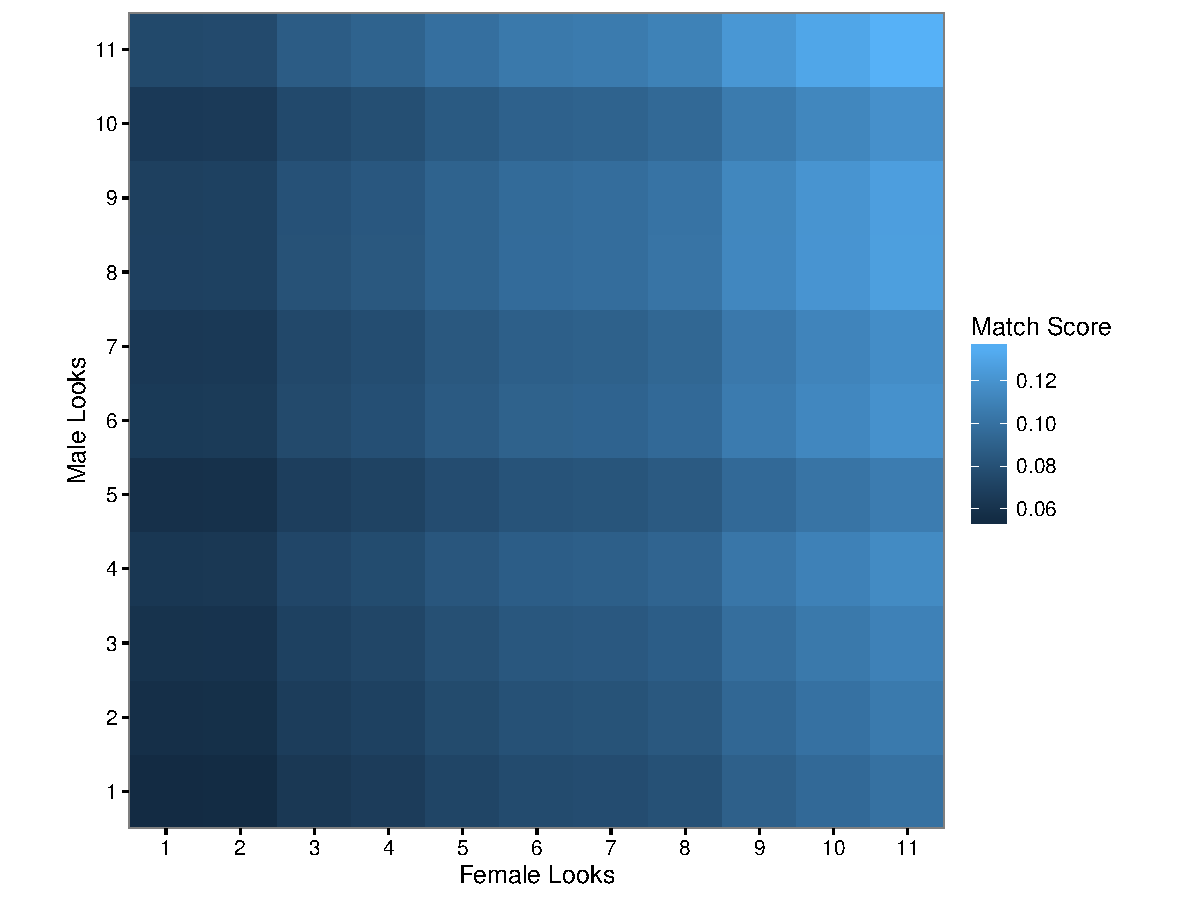
\includegraphics[scale=.7]{q3_score_heatmap.pdf}
  \label{fig:q3_score_heatmap}
\end{figure}

\begin{figure}[!htb]
  \centering
  \caption{Heatmap of Match-Scores by Male/Female Looks Using Both Sender \& Receiver Looks}
  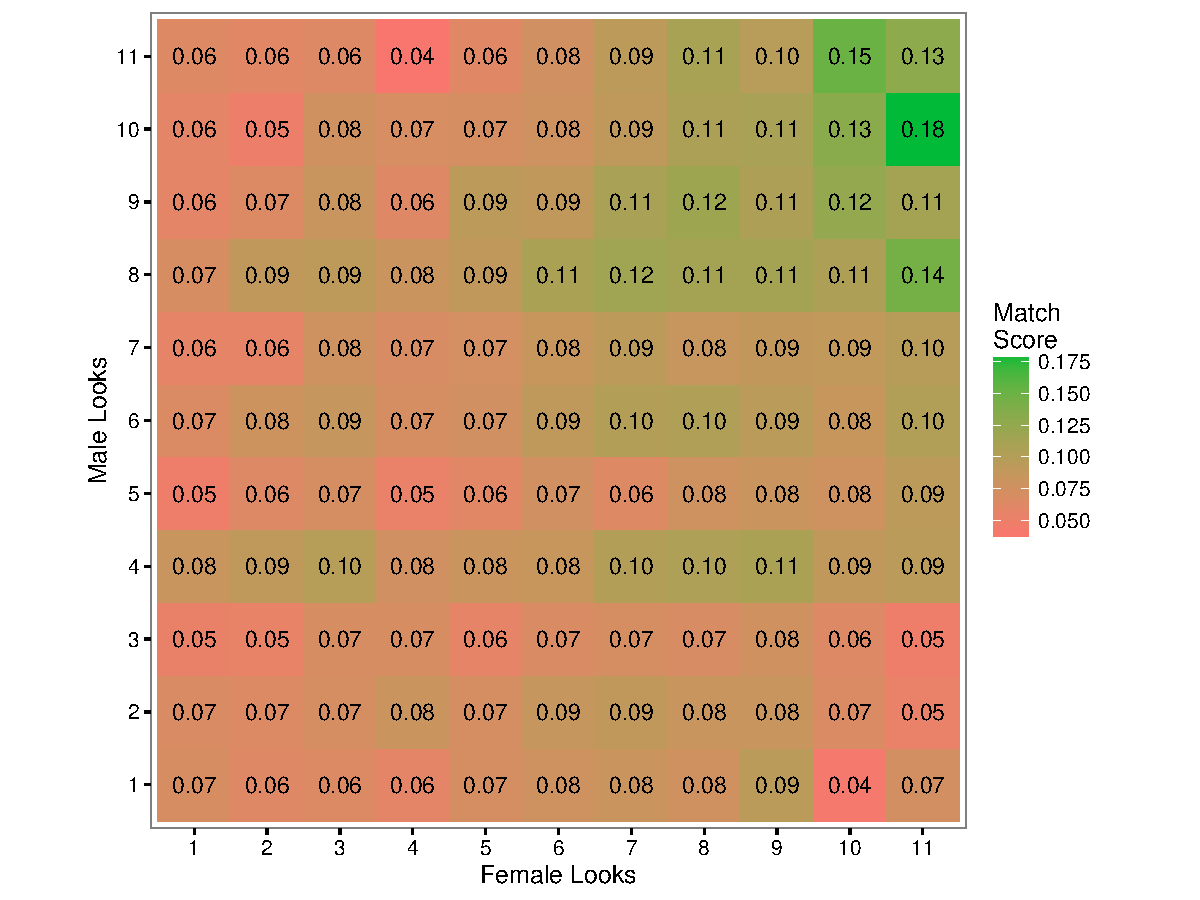
\includegraphics[scale=.7]{q4_heat.pdf}
  \label{fig:q4_heat}
\end{figure}

% \doublefig{Heatmap of Scores by Male/Female Looks}{q3_score_heatmap}{Using Receiver Looks Only}{q4_heat}{Using Both Sender \& Receiver Looks}


\section{}
First we regressed the binary contact indicator, \textit{y}, on \textit{ReceiverLooks}, \textit{SenderLooks}, and \textit{SenderGender} allowing those terms to interact with each other (see \vref{lst:q4_all}).  This took quite a while to run -- about 3 minutes on my 2010-era notebook -- and generated 242 coefficients ($11 * 11 * 2$).  While many of the coefficients were insignificant, they gave us a model we could use to account for sender/receiver looks as well as gender.  With this model, we then calculated a match score (see \vref{lst:q4_pred}) which we then used to generate a heat-map (see \vref{fig:q4_heat}).

\begin{lstlisting}[language=R,label=lst:q4_all,caption=Regressing y on all available data.]
glm(y ~ ReceiverLooks * SenderLooks * SenderGender, data=df, family="binomial")
\end{lstlisting}

\lstinputlisting[language=R,label=lst:q4_pred,caption=Predicting scores using all data.]{predict_snippet.R}

%%%%%%%%%%% BEGIN APPENDIX
\clearpage
\begin{appendices}

\crefalias{section}{appsec}
\section{Data Exploration} \label{app:1}

\singlefig{q0_data_heat}{}
\singlefig{q0_contact_heat}{}


\end{appendices}

\end{document}

% \input{.tex}

% \begin{figure}[!htb]
%   \centering
%   \caption{}
%   \begin{subfigure}[b]{0.49\textwidth}
%     \caption{}
%     \includegraphics[width=\textwidth]{.pdf}
%     \label{fig:}
%   \end{subfigure}
%   \hfill
%   \begin{subfigure}[b]{0.49\textwidth}
%     \caption{}
%     \includegraphics[width=\textwidth]{.pdf}
%     \label{fig:}
%   \end{subfigure}
% \end{figure}

% \begin{figure}[!htb]
%   \centering
%   \caption{}
%   \includegraphics[scale=.5]{.pdf}
%   \label{fig:}
% \end{figure}